\documentclass[conference]{IEEEtran}
\IEEEoverridecommandlockouts
% The preceding line is only needed to identify funding in the first footnote. If that is unneeded, please comment it out.
\usepackage{cite}
\usepackage{minted}
\usepackage{amsmath,amssymb,amsfonts}
\usepackage{algorithmic}
\usepackage{graphicx}
\usepackage{textcomp}
\usepackage{graphicx}
\usepackage{xcolor}
\ifCLASSOPTIONcompsoc
    \usepackage[caption=false, font=normalsize, labelfont=sf, textfont=sf]{subfig}
\else
\usepackage[caption=false, font=footnotesize]{subfig}
\fi

\def\BibTeX{{\rm B\kern-.05em{\sc i\kern-.025em b}\kern-.08em
    T\kern-.1667em\lower.7ex\hbox{E}\kern-.125emX}}
\begin{document}

\title{Ellipsoid Algorithm }

\author{\IEEEauthorblockN{Siddharth Bhat}
\IEEEauthorblockA{\textit{20161105}} \\
% \textit{name of organization (of Aff.)}\\
% City, Country \\
% email address}
%\and
%\IEEEauthorblockN{2\textsuperscript{nd} Given Name Surname}
%\IEEEauthorblockA{\textit{dept. name of organization (of Aff.)} \\
%\textit{name of organization (of Aff.)}\\
%City, Country \\
%email address}
%\and
%\IEEEauthorblockN{3\textsuperscript{rd} Given Name Surname}
%\IEEEauthorblockA{\textit{dept. name of organization (of Aff.)} \\
%\textit{name of organization (of Aff.)}\\
%City, Country \\
%email address}
%\and
%\IEEEauthorblockN{4\textsuperscript{th} Given Name Surname}
%\IEEEauthorblockA{\textit{dept. name of organization (of Aff.)} \\
%\textit{name of organization (of Aff.)}\\
%City, Country \\
%email address}
%\and
%\IEEEauthorblockN{5\textsuperscript{th} Given Name Surname}
%\IEEEauthorblockA{\textit{dept. name of organization (of Aff.)} \\
%\textit{name of organization (of Aff.)}\\
%City, Country \\
%email address}
%\and
%\IEEEauthorblockN{6\textsuperscript{th} Given Name Surname}
%\IEEEauthorblockA{\textit{dept. name of organization (of Aff.)} \\
%\textit{name of organization (of Aff.)}\\
%City, Country \\
%email address}
}

\newcommand{\PTIME}{\texttt{PTIME}}
\maketitle

\begin{abstract}
We motivate the Ellipsoid algorithm, discuss its original theoretical
importance, and remark on its practical efficiency.
\end{abstract}

\begin{IEEEkeywords}
component, formatting, style, styling, insert
\end{IEEEkeywords}

\section{Introduction}
The ellipsoid algorithm was discovered in Naum Z. Shor. Later, 
Leonid Genrikhovich Khachiyan proved that the algorithm runs in polynomial
time. This was a breakthrough in the theory of linear programming, which
proved that solving LP's is in \PTIME.

\section{High level description the algorithm: Checking for non-emptiness}
The ellipsoid algorithm is an algorithm that allows us to check for the
non-emptiness of a system of linear equations. 


An \textit{ellipsoid} in $\mathbb{R}^n$ is a set of points
\[E \equiv \left\{ (x_1, x_2, \dots x_n) \mid \sum_i \frac{x_i^2}{a_i^2} \leq 1 \right\}\] for some
constants $(a_1, a_2, \dots a_n)$. 

The algorithm works by first bounding the polyhedra $P \equiv \{ x | Ax \leq b \}$ 
with a large initial bounding ellipsoid, such that $P \subset E_0$. We now pick a
random point $p \in E_0$, and check if this point is in the polyhedra $P$. If it
is, then we are done, as we have found a feasible point $p \in P$. On the
other hand, if $p \notin P$, we shrink the ellipsoid $E_0$ to a smaller
ellipsoid $E_1$ such that $p \notin E_1$, but $P \subseteq E_1$. That is,
we shrik the ellipsoid such that the point $p$ is no longer in the ellipsoid,
but the polyhedra still is. We then repeat the process.

Now, of course, one can imagine this process going on forever, since perhaps
our polyhedra $P$ truly is empty, but we keep picking points in our ellipsoids,
since our ellipsoid as described above can never shrink to the empty set.

To prevent this case, we are also given a \textit{lower bound} $V_l$ on the volume
of the polyhedra. Now, after some iteration, if the volume of the ellipsoid $Vol(E)$
goes below $V_l$, we can conclude that $P \not\subseteq E$. Thus, we can
terminate with infeasibility.

Thus, for this algorithm to work, the main ingredients are:
\begin{itemize}
\item The polyhedra $P \equiv \{ x | Ax \leq b \}$ whose non-emptiness
                is to be tested.
\item The initial ellipsoid $E_0$ that bounds $P$ of volume $V_u$.
\item The lower bound on the volume of $P$, $V_l$ such that $0 < V_l \leq
        Vol(P)$. 
\item An algorithm which when given a point $x$ and the polyhedra $P$, either
        certifies $x \in P$, or provides us information about how to separate
                $x$ from $P$, so we can shrink our ellipsoid.
\end{itemize}

Given these ingredients, we show how to construct the algorithm.  We show later
in the report how this can be used to solve LP's in polynomial time. Here, we
present a specific version of the Ellipsoid algorithm. The more general version
works over convex sets, and requires a gadget known as a \textit{separation
oracle} which provides us the separation information of $x$ from $P$. In the
case of LP, this gadget reduces to the Farkas' Lemma. So, we shall proceed to
discuss the algorithm for the LP case only.

\begin{figure}
    \subfloat[iteration 0]{ 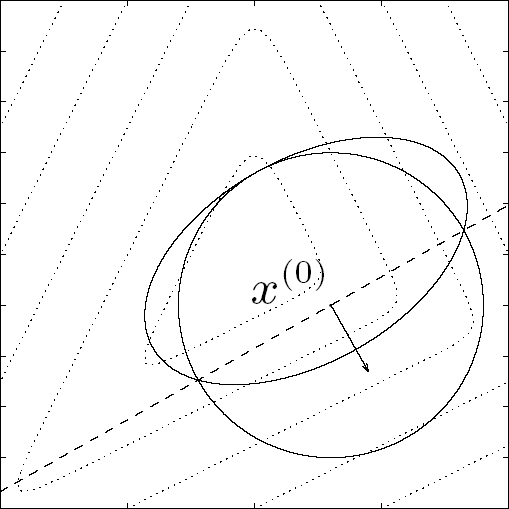
\includegraphics[width=.4\linewidth]{e1.png}}
    \subfloat[iteration 1]{ 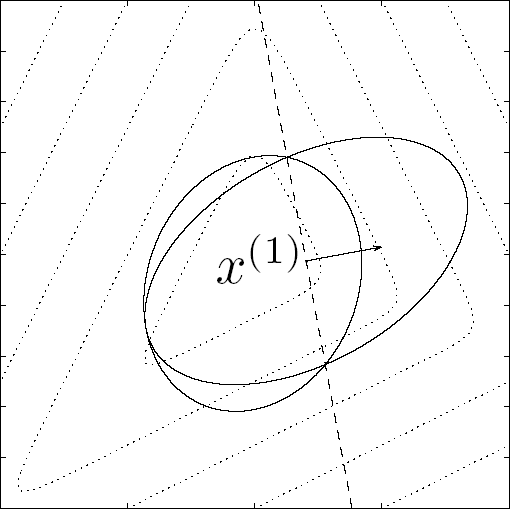
\includegraphics[width=.4\linewidth]{e2.png}}
    \\
    \subfloat[iteration 2]{ 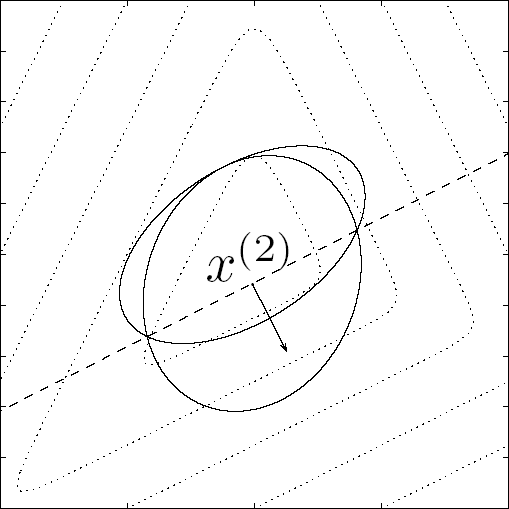
\includegraphics[width=.4\linewidth]{e3.png}}
    \subfloat[iteration 3]{ 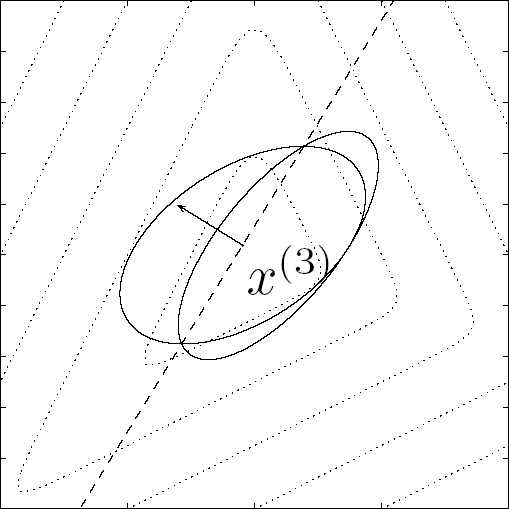
\includegraphics[width=.4\linewidth]{e4.png}}
    \\
    \subfloat[iteration 4]{ 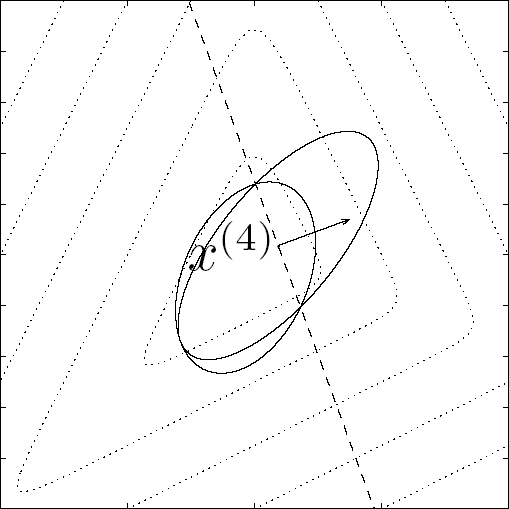
\includegraphics[width=.4\linewidth]{e5.png}}
    \subfloat[iteration 5]{ 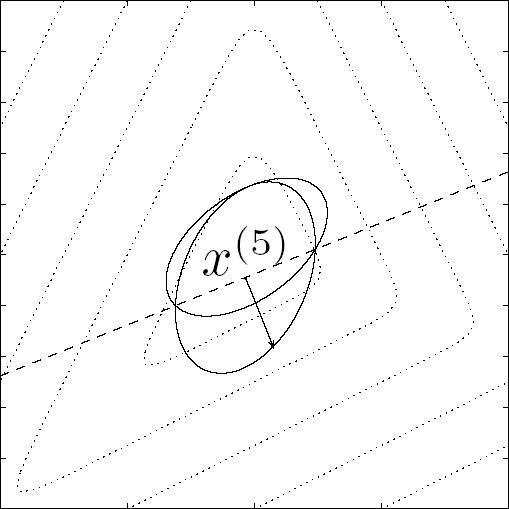
\includegraphics[width=.4\linewidth]{e6.png}}
\caption{Sequence of iteration of ellipsoid method}
\end{figure}




\section{Using non-emptiness to solve LP's}
So far, all we can do using the ellipsoid algorithm is to check if some
system of equations $Ax \leq b$ is \textit{non-empty}. In other words, we
can check the non-emptiness of a given polyhedron. Here, we will describe how
to use this to solve \textit{optimisation problems}.

Consider a linear program and its dual:
\begin{align*}
        &x, c \in \mathbb R^{n \times 1} \quad A \in \mathbb R^{m \times n} \quad b, y \in \mathbb R^{m \times 1}\\
        &P_{primal} \equiv \underset{x}{\text{maximise }} c^T x \text{ subject to } Ax = b \\
        &P_{dual} \equiv \underset{y}{\text{minimise }} b^T y \text{ subject to } A^Ty \geq c \quad
\end{align*}

Let $x^\star$ be the optimal value of $x$ for $P_{primal}$, and $y^\star$ be the
optimal value of $y$ for $P_{dual}$. From strong duality, we know that
the value of $c^Tx^\star = b^Ty^\star$.

So, we can create a \textit{combined} linear program, whose feasibility will
force us to provide a point such that $c^Tx = b^T y$. That is, we create
a new polyhedra $Q$ defined by the equations:

\begin{align*}
        A x \leq b \quad
        A^T y \geq c \quad
        c^Tx = b^T y
\end{align*}

Now, if a feasible point $(x_0, y_0) \in Q$, then it must be the case that $Ax_0 = b$,
$A^Ty_0 \geq c$, and $c^Tx_0 = b^Ty_0$. At this point, strong duality tells us that
$(x_0, y_0) = (x^\star, y^\star)$. 

Hence, we can find the optimal value of the linear program by evaluating $c^T x_0$.


Thus, the ellipsoid algorithm can be used to solve for the optimality of a linear
program, by starting from a non-emptiness check! This is beautiful, and proves
a deep result of LP's: A certificate of non-emptiness is as good as a ceritificate
of optimality.

\section{Proof that ellipsoid algorithm is polynomial in input size}
Here, we sketch the proof that the ellipsoid algorithm is polynomial
in its input size.

The minimum volume ellipsoid that surrounds a half-ellipsoid $E_i \cap H^+$ can
be calculated in polynomial time, and:

\begin{align*}
V(E_{i+1}) \leq (1 - \frac{1}{2n}) V(E_i)
\end{align*}

This comes from a non-trivial lemma of convex geometry.

If the loop in the algorithm runs $t$ times, then by the above lemma:

\begin{align*}
    \left( 1 - \frac{1}{2n} \right)^t \leq \frac{V_u}{V_l} \implies t = O(n \log \frac{V_u}{V_l})
\end{align*}

\section{Code implementing the algorithm}
The code is written using the SAGE mathematical system, which provides a rich
library for polyhedra. This allows one to prototype geometric algorithms
with very little code. The code can be run by executing it with \texttt{sage program.py},
and is presented in figure \ref{fig:code}

\begin{figure}[!htb]
\inputminted{py}{ellipsoid.sage}
\caption{Implementation of the ellipsoid algorithm in SAGE}
\label{fig:code}
\end{figure}

A sample run is shown below:
\inputminted[fontsize=\footnotesize]{text}{ellipsoid-output}


\bibliographystyle{IEEEtran}
\bibliography{references.bib}

\end{document}
